\documentclass[12pt,aspectratio=169]{beamer}
\usetheme{metropolis}
\setbeamersize{text margin left=.5cm,text margin right=.5cm}
\usepackage[lf]{carlito}
\usepackage{siunitx}
\usepackage{tikz}
\usepackage{mathpazo}
\usepackage{bm}
\usepackage{mathtools}
\usepackage[ISO]{diffcoeff}
\diffdef{}{ op-symbol=\mathsf{d} }
\usepackage{xcolor,colortbl}

\setmonofont{Ubuntu Mono}
\setlength{\parskip}{0pt}
\renewcommand{\baselinestretch}{1}

\sisetup{
  inter-unit-product=\cdot,
  per-mode=symbol
}

\tikzset{
  >=latex
}

%\newcommand{\iii}{\hat{\bm\imath}}
%\newcommand{\jjj}{\hat{\bm\jmath}}
%\newcommand{\kkk}{\hat{\bm k}}


\title{Class 16: Capacitors}
\subtitle{Advanced Placement Physics C}
\author[TML]{Dr.\ Timothy Leung}
\institute{Olympiads School}
\date{Updated: Summer 2022}

\newcommand{\pic}[2]{
  \includegraphics[width=#1\textwidth]{#2}
}
\newcommand{\eq}[2]{
  \vspace{#1}{\Large
    \begin{displaymath}
      #2
    \end{displaymath}
  }
}
%\newcommand{\iii}{\ensuremath\hat{\bm{\imath}}}
%\newcommand{\jjj}{\ensuremath\hat{\bm{\jmath}}}
%\newcommand{\kkk}{\ensuremath\hat{\bm{k}}}
\newcommand{\iii}{\ensuremath\hat\imath}
\newcommand{\jjj}{\ensuremath\hat\jmath}
\newcommand{\kkk}{\ensuremath\hat k}



\begin{document}

\begin{frame}
  \maketitle
\end{frame}


\section{Parallel-Plate Capacitors}

\begin{frame}{Electric Field and Electric Potential Difference}
  Recall that the relationship between electrostatic force ($\vec F_q$) and
  electric potential energy ($U_q$) can be expressed using definition of
  mechanical work and the fundamental theorem of calculus:

  \eq{-.1in}{
    \Delta U_q=-\int\vec F_q\cdot\dl\vec r\quad\quad
    \vec F_q=-\nabla U_q=-\diffp{U_q}r\hat r
  }

  Dividing both sides of the equations by $q$, we get the relationship between
  electric field ($\vec E$), electric potential ($V$) and electric potential
  difference ($\Delta V$):
  
  \eq{-.1in}{
    \Delta V=-\int\vec E\cdot\dl\vec r\quad\quad
    \boxed{\vec E=-\nabla V=-\diffp Vr\hat r}
  }

  This relationship holds regardless of the charge configuration.
\end{frame}



\begin{frame}{Electric Field and Electric Potential Difference}
  \begin{center}
    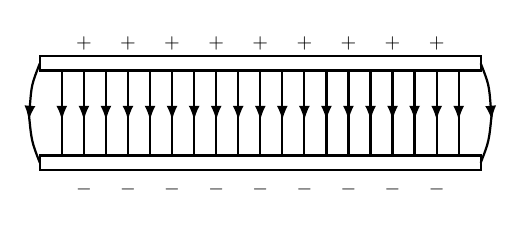
\begin{tikzpicture}[xscale=.7,yscale=.9]
      \draw[thick] rectangle (8,.2);
      \draw[thick](0,1.4) rectangle (8,1.6);
      \foreach\x in {.4,.8,1.2,...,7.6}{
        \draw[->,thick](\x,1.4)--(\x,.7);
        \draw[thick](\x,1.4)--(\x,.2);
      }
      \foreach\x in {.8,1.6,2.4,...,7.2}{
        \node at (\x,1.78) {\scriptsize $+$};
        \node at (\x,-.28) {\scriptsize $-$};
      }
      
      \draw[->,thick](0,1.5)..controls(-.15,1.2)..(-.2,.7);
      \draw[thick](-.2,.8)..controls(-.15,.4)..(0,.1);

      \draw[->,thick](8,1.5)..controls(8.15,1.2)..(8.2,.7);
      \draw[thick](8.2,.8)..controls(8.15,.4)..(8,.1);
    \end{tikzpicture}
  \end{center}
  Recall that for two charged parallel plates, the electric field is uniform,
  and the relationship between electric field and potential difference
  simplifies to:

  \eq{-.1in}{
    \boxed{E=\frac{\Delta V}d}
    \quad\text{or}\quad
    \boxed{\Delta V=Ed}
  }
\end{frame}



\begin{frame}{Capacitors}
  \textbf{Capacitors} is a device that stores energy in an electric field. The
  simplest form of a capacitor is a set of closely spaced parallel plates:
  \begin{center}
    \pic{.5}{cap19}
  \end{center}
  When the plates are connected to a battery, the battery transfer charges to
  the plates until the voltage $V$ equals the battery terminals. After that,
  one plate has charge $+Q$; the other has $-Q$.
\end{frame}



\begin{frame}{Parallel-Plate Capacitors}
  As we have seen already, the (uniform) electric field between two parallel
  plates is proportional to the charge density $\sigma$, which is the charge
  $Q$ divided by the area of the plates $A$:

  \eq{-.1in}{
    E=\frac{\textcolor{red}{\sigma}}{\epsilon_0}=
    \frac{\textcolor{red}{Q}}{\textcolor{red}{A}\epsilon_0}
  }
  
  Substituting this into the relationship between the plate voltage $V$ and
  electric field, we find the relationship between the charges across the
  plates and the voltage:

  \eq{-.1in}{
    \Delta V=\textcolor{blue} Ed=
    \frac{\textcolor{blue}{Q}d}{\textcolor{blue}{A\epsilon_0}}
    \quad\longrightarrow\quad
    \boxed{Q=\left[\frac{A\epsilon_0}d\right]\Delta V}
  }
\end{frame}



\begin{frame}{Parallel-Plate Capacitors}
  Since area $A$, distance of separation $d$ and the vacuum permittivity
  $\epsilon_0$ are all constants, the relationship between charge $Q$ and
  voltage $\Delta V$ is \emph{linear}. The constant is called the
  \textbf{capacitance} $C$, defined as:

  \eq{-.1in}{
    \boxed{C=\frac Q{\Delta V}}
  }

  For parallel plates:

  \eq{-.1in}{
    \boxed{C=\frac{A\epsilon_0}d\quad\text{parallel plate}}
  }

  The unit for capacitance is a \textbf{farad} (named after Michael Faraday),
  where $\SI1\farad=\SI1{\coulomb\per\volt}$.
\end{frame}



\begin{frame}{Storage of Electrical Energy}
  When charging up a capacitor, imagine positive charges moving from the
  negatively charged plate to the positively charged plate
  \begin{center}
    \pic{.45}{slide14}
  \end{center}
  %Initially neither plates are charged, so moving the first charge takes very
  %little work; as the electric field builds, more and more work needs to be
  %done
\end{frame}



\begin{frame}{Storage of Electrical Energy}
  \begin{center}
    \pic{.35}{slide14}
  \end{center}
  In the beginning---when the plates aren't charged---moving an infinitesimal
  charge $\dl q$ across the plates, the infinitesimal work done $\dl U$ is very
  small and related to the capacitance by:

  \eq{-.1in}{
    \dl U=V\dl q=\frac qC\dl q
  }
  
  As the electric field begins to form between plates, more and more work
  is required to move the charges.
\end{frame}



\begin{frame}{Storage of Electrical Energy}
  To fully charge the plates, the total work $U_c$ is the integral:

  \eq{-.1in}{
    U_c=\int\dl U=\int_0^Q\frac qC\dl q=\frac12\frac{Q^2}C
  }

  The work done is stored as a potential energy inside the capacitor. There are
  different ways to express $U_c$ using definition of capacitance:

  \eq{-.1in}{
    \boxed{U_c=\frac12\frac{Q^2}C=\frac12QV=\frac12CV^2}
  }
\end{frame}


\section{Cylindrical Capacitors}

\begin{frame}{Cylindrical Capacitors}
  \begin{columns}
    \column{.4\textwidth}
    \pic{1.05}{cylindrical-capacitor}

    \column{.56\textwidth}
    Not all capacitors are parallel plates. Cylindrical capacitors are also
    popular.
    \begin{itemize}
    \item The capacitor has length $\ell$ which is much larger than the radii
      of the inner \& outer cylinders ($a$, $b$)
    \item Inner cylinder has total charge $Q$
    \item Outer cylinder has total charge $-Q$
    \item Inside the capacitor, the electric field in the radial direction
    \item Outside of the capacitor, there is no electric field
    \end{itemize}
  \end{columns}
\end{frame}



\begin{frame}{Cylindrical Capacitors: Electric Field}
  \begin{columns}
    \column{.4\textwidth}
    \pic{1.05}{cylindrical-capacitor}

    \column{.56\textwidth}
    Use Gauss's law to find the electric field between the cylinders, by placing
    a Gaussian surface of radius $r$ between the cylinders: 

    \eq{-.1in}{
      \oint\vec E\cdot\dl\vec A=2\pi r\ell E=\frac Q{\epsilon_0}
    }
    
    which gives the expression:

    \eq{-.1in}{
      E=\frac Q{2\pi r\ell\epsilon_0}\quad\text{or}\quad
      E=\frac\lambda{2\pi r\epsilon_0}
    }
    
    where $\lambda=Q/\ell$ is the linear charge density
  \end{columns}
\end{frame}




\begin{frame}{Cylindrical Capacitors: Voltage Across the Cylinders}
  Integrating the eclectic field to get voltage across the plates:

  \eq{-.1in}{
    \Delta V= \int_a^b E\dl r=\frac Q{2\pi\ell\epsilon_0}\int_b^a\frac{\dl r}r
    =\frac Q{2\pi\ell\epsilon_0}\ln\left[\frac ba\right]
  }

  Like parallel plates, the relationship between voltage and charge is still
  linear, but in this case, the capacitance is defined as:

  \eq{-.1in}{
    C=\frac Q{\Delta V}=\frac{2\pi\ell\epsilon_0}{\ln(b/a)}
    \quad\longrightarrow\quad
    \boxed{\frac C\ell=\frac{2\pi\epsilon_0}{\ln(b/a)}\;\;\text{cylindrical}}
  }

  The capacitance is generally expressed by $C/\ell$ (with unit
  \si{\farad\per\metre}). Like the parallel-plate capacitor, the capacitance of
  the cylindrical capacitor also only depends on the geometry (i.e.\ the raidii
  $a$ and $b$) and the permittiviy.
\end{frame}



\begin{frame}{Capacitance}
  Regardless of the geometry of the capacitor, the electric field will always
  be proportional to the charge, i.e.:

  \eq{-.2in}{ E\propto Q }

  and therefore the voltage will always be proportional to charge as well.
\end{frame}



\section{Practical Capacitors}

\begin{frame}{Practical Capacitors}
  \begin{columns}
    \column{.3\textwidth}
    \pic{1.15}{Figure_20_05_05a}

    \column{.7\textwidth}
    \begin{itemize}
    \item Capacitors (both parallel-plate and cylindrical) are very common in
      electric circuits, but the vacuum between the plates is not very effective
    \item Instead, a non-conducting \textbf{dielectric} material is inserted
      between the plates
    \item When the plates are charged, the electric field of the plates
      polarizes the dielectric.
    \item The polarization  produces an electric field that opposes the field
      from the plates, therefore reduces the effective voltage, and increasing
      the capacitance
    \end{itemize}
  \end{columns}
\end{frame}



\begin{frame}{Dielectric Constant}
  If electric field without dielectric is $E_0$, then $E$ in the dielectric is
  reduced by $\kappa$, the \textbf{dielectric constant}:

  \eq{-.1in}{
    \boxed{\kappa=\frac{E_0}E}
  }

  The capacitance of the plates with the dielectric is now amplified by the
  same factor $\kappa$:

  \eq{-.1in}{
    \boxed{C=\kappa C_0}
  }

  We can also view the dielectric as something that increases the
  \emph{effective permittivity}:
  
  \eq{-.1in}{
    \boxed{\epsilon=\kappa\epsilon_0}
  }
\end{frame}



\begin{frame}{Dielectric Constant}
  The dielectric constants of commonly used materials are:
  \begin{center}
    \begin{tabular}{l|l}
      \rowcolor{pink}
      \textbf{Material} & $\kappa$ \\ \hline
      Air         & \num{1.00059} \\
      Bakelite    & \num{4.9} \\
      Pyrex glass & \num{5.6} \\
      Neoprene    & \num{6.9} \\
      Plexiglas   & \num{3.4} \\
      Polystyrene & \num{2.55} \\
      Water (\SI{20}\celsius) & \num{80} 
    \end{tabular}
  \end{center}
\end{frame}



\begin{frame}{Notes About Storage of Electric Energy}
  The work done (i.e.\ the energy stored in the capacitor) is inversely
  proportional to the capacitance:

  \eq{-.1in}{
    \dl U=V\dl q=\frac qC\dl q
  }

  \begin{itemize}
  \item The presence of a dielectric \emph{increases} the capacitance; therefore
    the work (and potential energy stored) to move the charge $\dl q$
    \emph{decreases} with the dielectric constant $\kappa$
  \item After the capacitor is charged, removing the dielectric material from
    the capacitor plates will require additional work.
  \end{itemize}
\end{frame}



\begin{frame}{Capacitors in Electric Circuits}
  Capacitors are an important part of an electric circuits because it stores
  energy in the electric field. Suppose we replace a battery with a capacitor
  in a basic resistive circuit:
  \begin{center}
    \begin{tikzpicture}[scale=.85]
      \draw[thick](0,0) to[C=$C$] (0,3)--(3,3) to[R=$R$] (3,0)--(0,0);
    \end{tikzpicture}
  \end{center}
  \begin{itemize}
  \item The capacitor acts like a voltage source.
  \item Unlike a battery, the voltage decreases as it drives a current, and the
    charge across the capacitor plates decreases.
  \end{itemize}
\end{frame}
\end{document}
